\section{Objects and Maps}% {{{
\label{sec:objects_and_maps}

\twocolumn
\subsection{Objects}%
\label{sub:objects}

\subsubsection{IV drip}%
\label{ssub:iv_drip}

When the patients wake up they're hooked up to IV drips, which can be used as makeshift weapons with reach, dealing \redbf{2 Harm}
on a full success.

\subsubsection{Keycard}%
\label{ssub:keycard}

The orderly has a \textbf{keycard} that opens every locked door in the ward.
\begin{figure}[!htbp]
  \includegraphics[height=5.5cm, keepaspectratio]{resources/img/keycard.png}
  \caption{Orderly's keycard}\label{keycard}
\end{figure}

\subsubsection{Pistol}%
\label{ssub:pistol}

\begin{figure}[!htbp]
  \includegraphics[width=5.5cm, keepaspectratio]{resources/img/glock.png}
  \caption{Pistol found in the only locked locker in the \textbf{staff room}}\label{pistol}
\end{figure}
The gun belonged to the security guard, before he was turned into what he is now.  There is also a driver's license in the
locker belonging to a Benjamin K. Miller, and the photo shows someone very similar looking to the
\hyperref[ssub:orderly]{orderly}, less bloated and grey though.


\subsubsection{Vials}%
\label{ssub:vials}

\begin{figure}[!htbp]
  \centering
  \includegraphics[width=5.5cm, keepaspectratio]{resources/img/test tubes.png}
  \caption{Vials of spinal fluid extracted for experimentation}\label{vials}
\end{figure}
These vials can be found in the fridge in the laboratory, four of them have their name and room number attached.  When they are
taken out and not put in a cooler they are starting to develop black flakes like ash or grime, while at the same time fingers
or toes go numb and start to blacken with necrosis.  If they are not put back into cold storage in time characters will incur
\redbf{1 Serious Wound} that can be stabilised by putting the vials in a cold place for a while.

When one of these vials is destroyed the PC named on the vial just dies instantaneously, which allows their spirit to leave the
body.  This will cost them \redbf{-2 Stability} for the traumatic experience of dying.  The PC's spirit can now try to find a new
body in one of the \hyperref[ssub:other_patient_rooms]{other patient rooms}~(p.~\pageref{ssub:other_patient_rooms}).

\subsubsection{Documents}%
\label{ssub:documents}

\begin{figure}[!htbp]
  \centering
  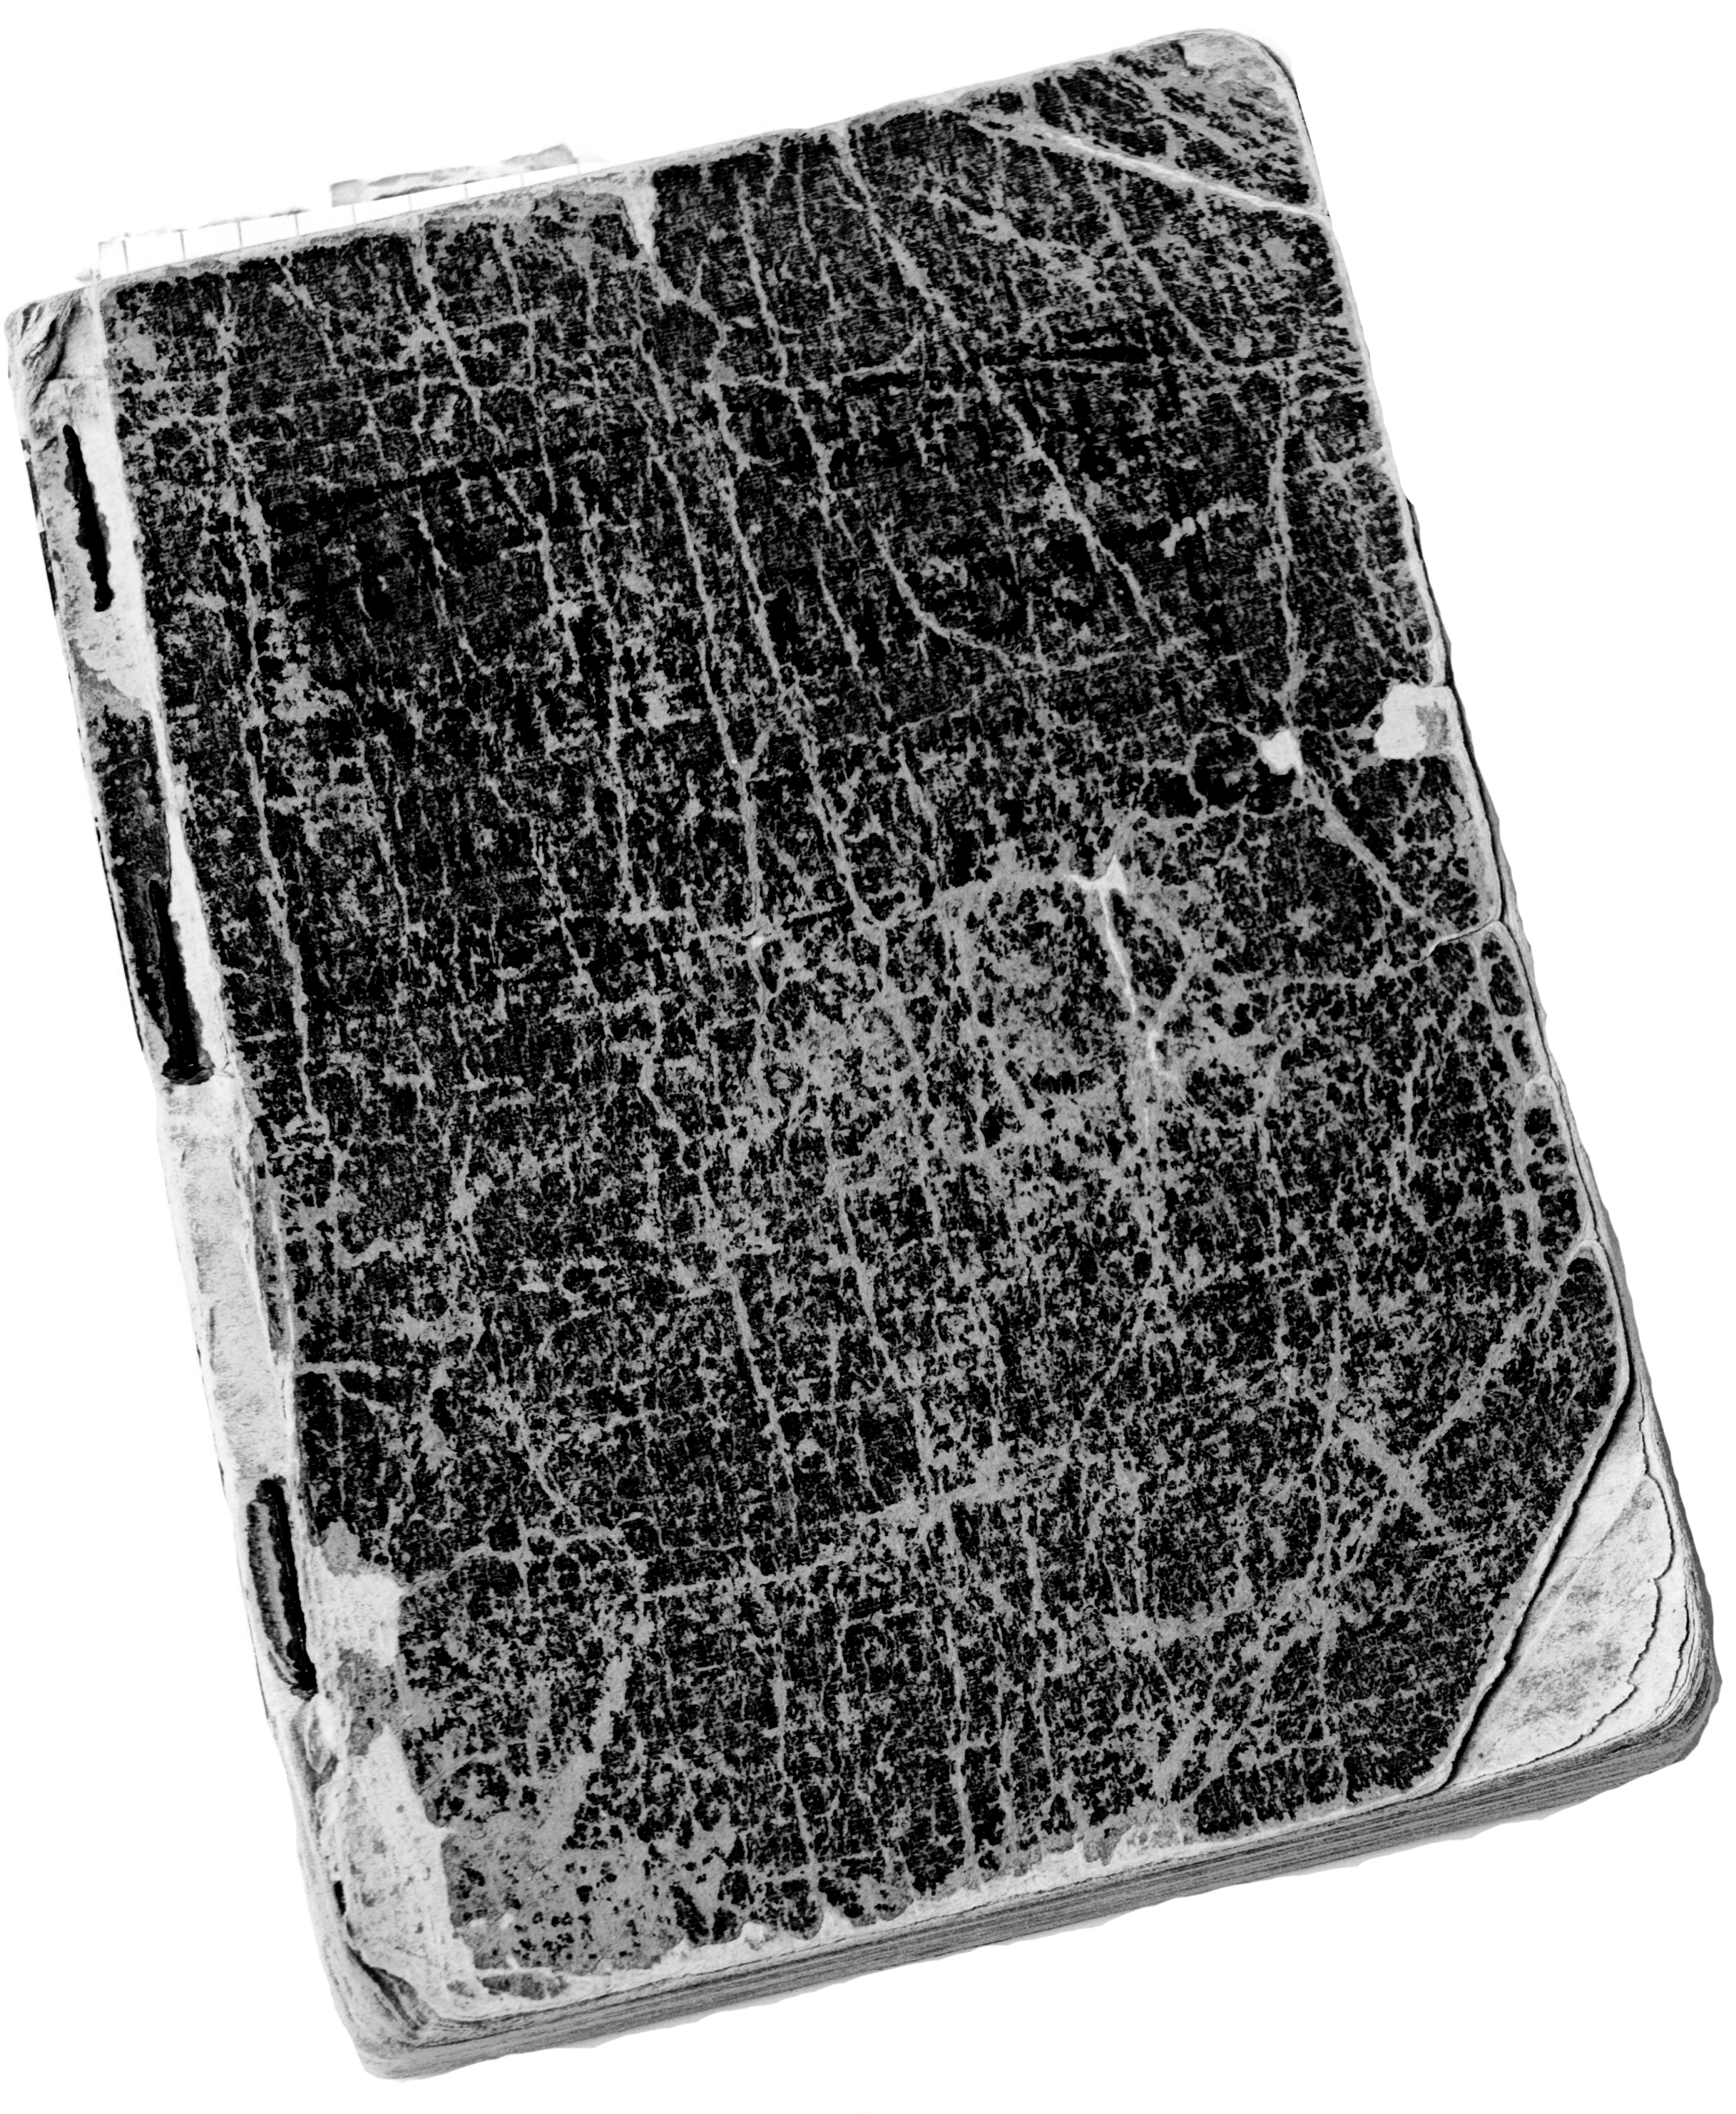
\includegraphics[width=5.5cm, keepaspectratio]{resources/img/journal.png}
  \caption{Joanna O'Banion's journal with the “experimental” procedures}\label{notebook}
\end{figure}

\clearpage
\onecolumn
\subsection{Map}%
\label{sub:map}
\hspace*{-0.5cm}%
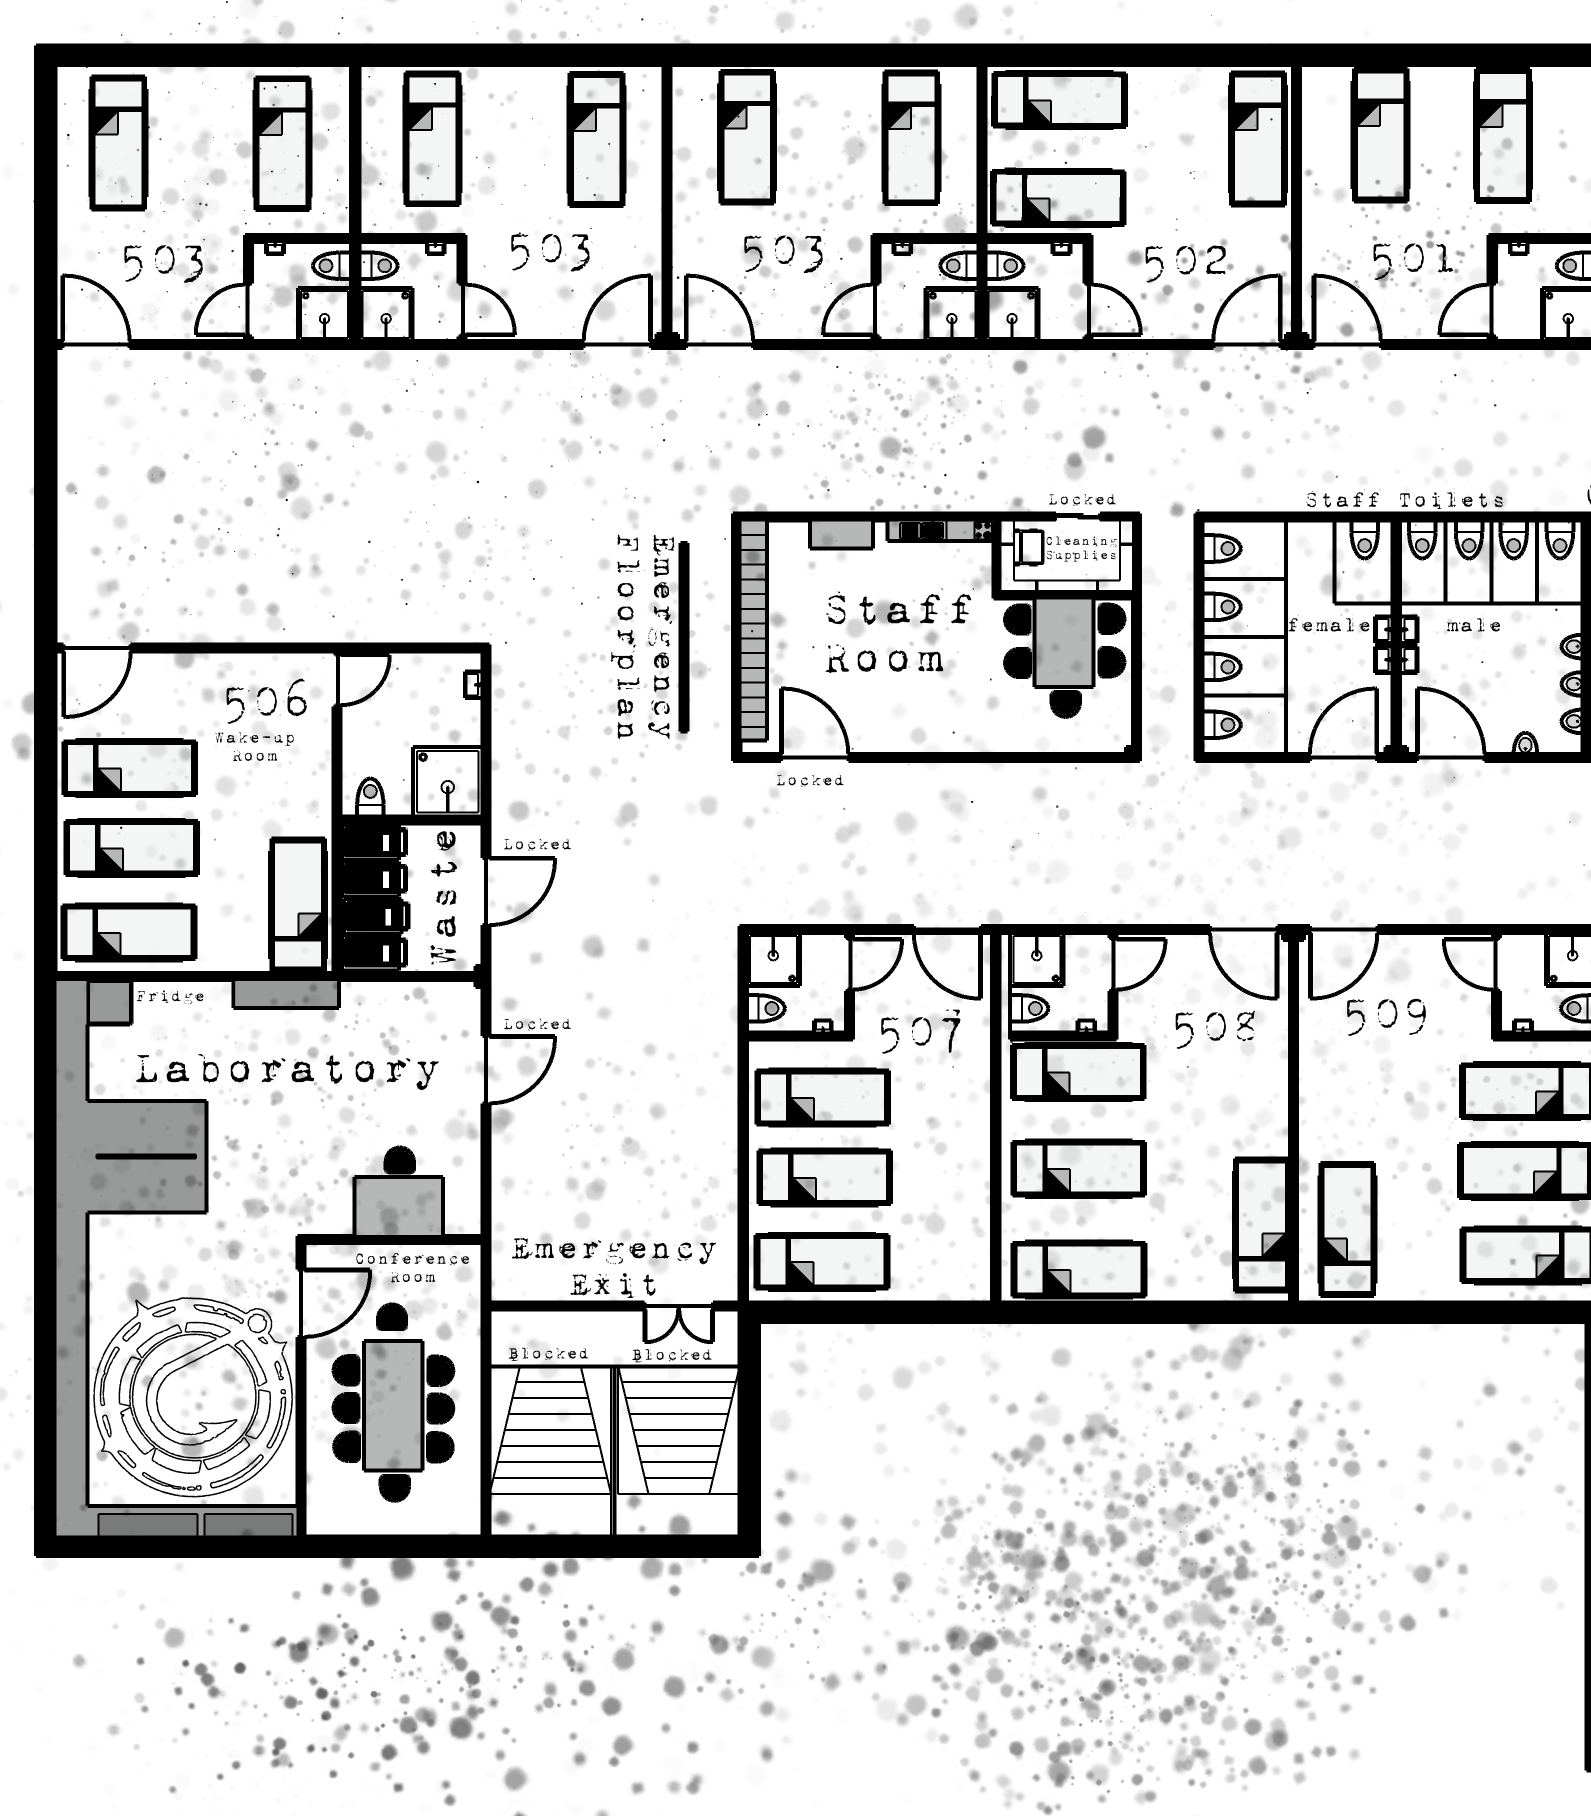
\includegraphics[width=19.5cm, keepaspectratio]{resources/img/the ward-gm-L.png}
\newpage
\vspace*{0.55cm}%
\hspace*{-2.0cm}%
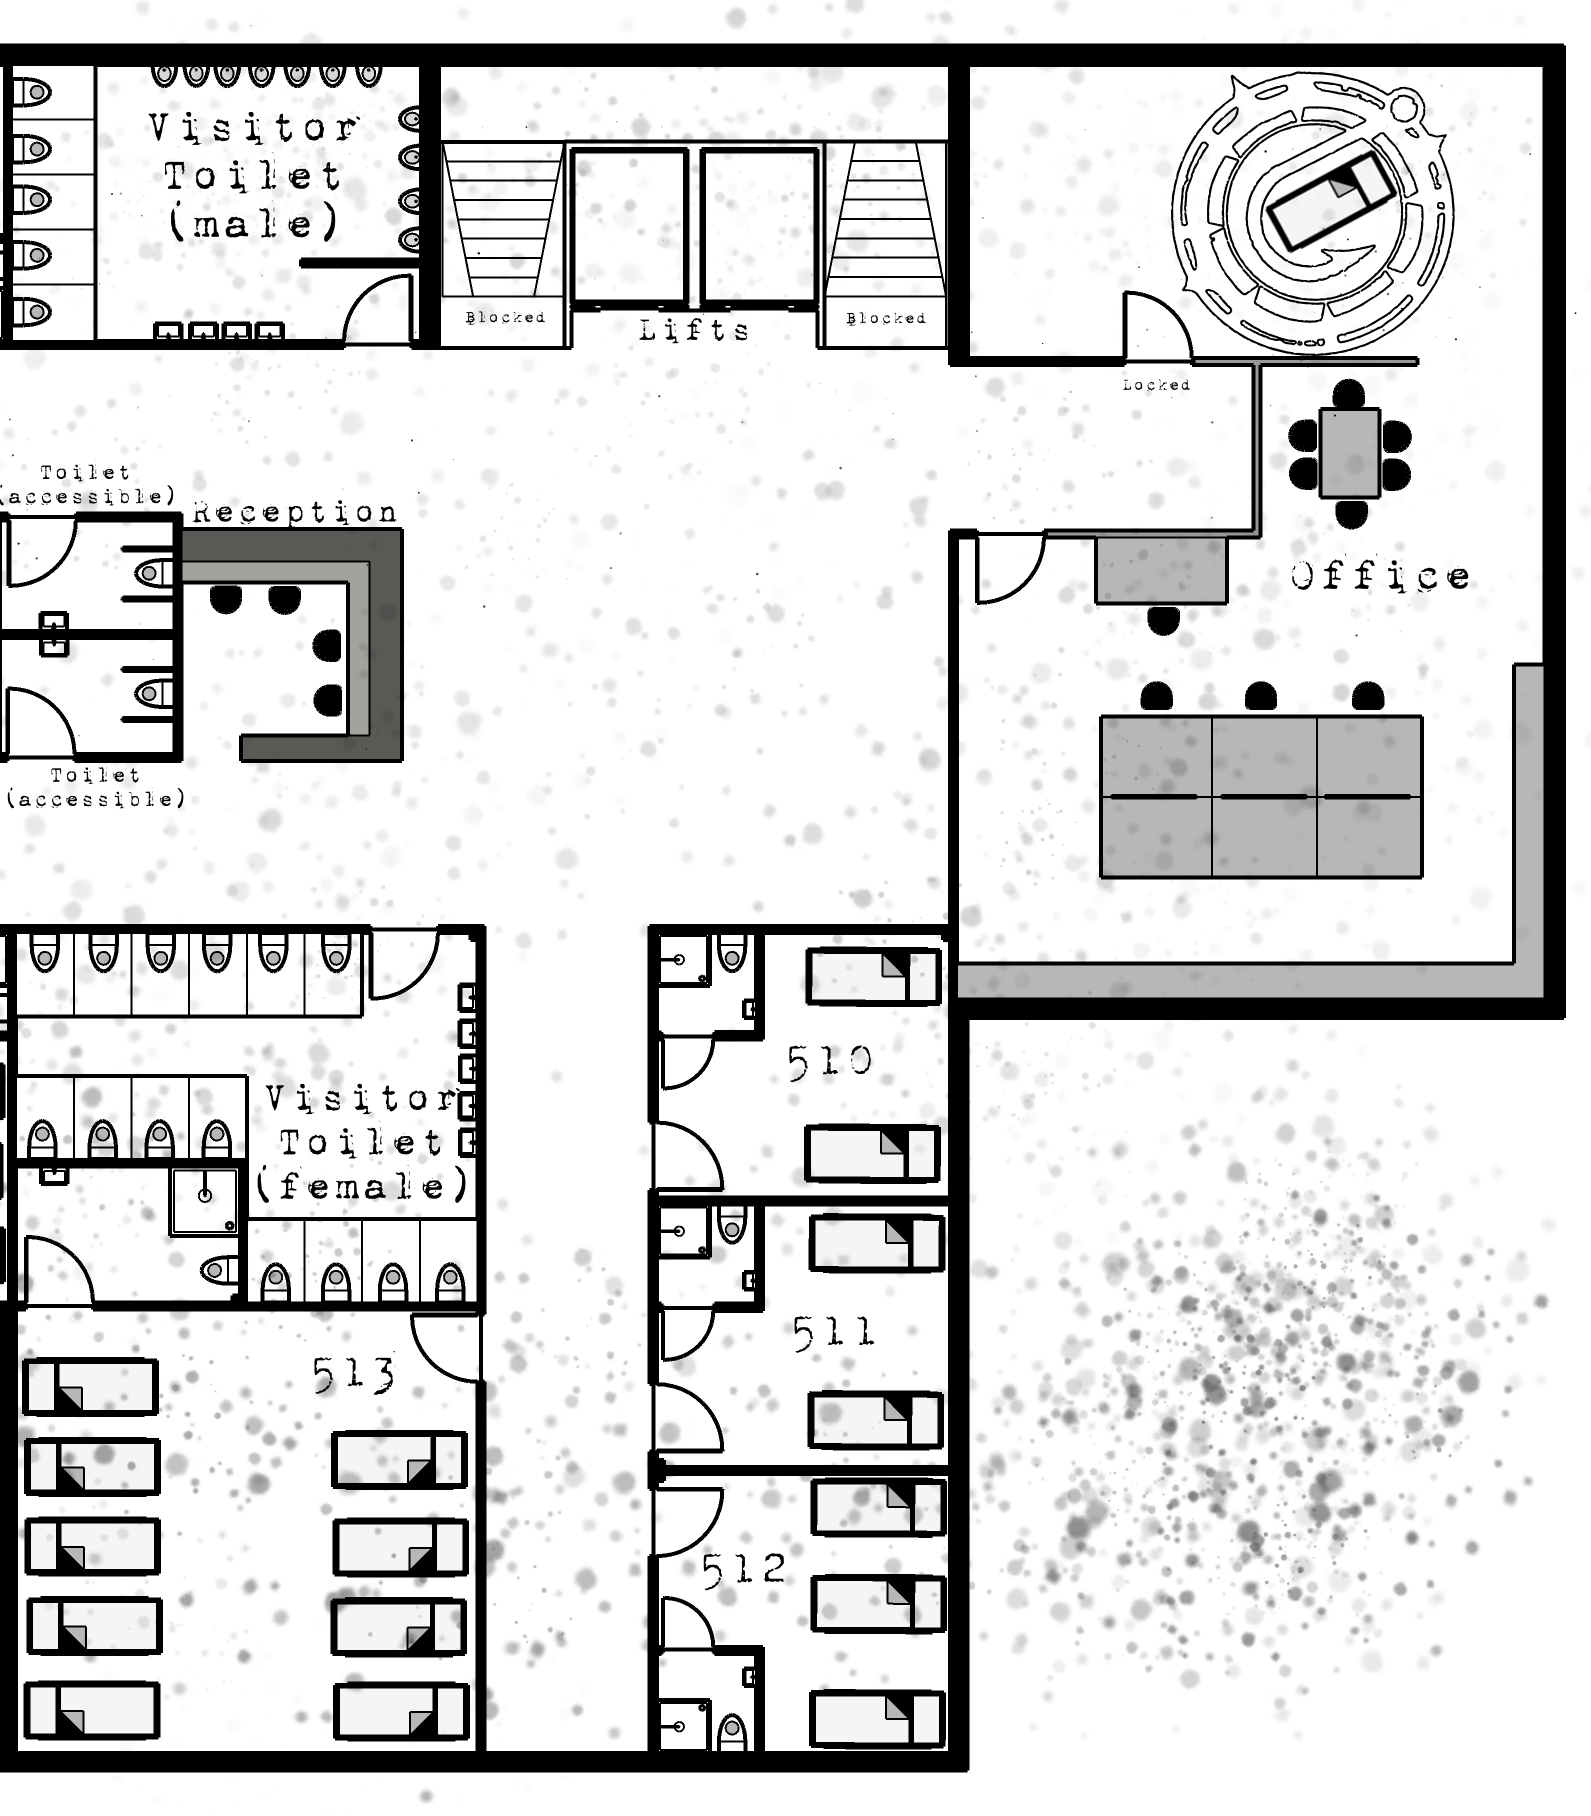
\includegraphics[width=19.5cm, keepaspectratio]{resources/img/the ward-gm-R.png}
\clearpage % }}}

